\chapter{Removing host dependency for optimization}
\label{cha:sys_fpgaonly}

The timestepping loops which are dependent on the size of the meshes are present in the host.
Every iteration, the host uses the helper class \texttt{kernel\_group} method
\texttt{enqueue\_NDRange()} to enqueue the subgroup of the kernels to perform the
computation for that timestep and synchronize the kernel execution to sequentially
execute the kernels on non-shared elements followed by shared elements after the completion
of data transfers. This requires two host interactions per iteration, one each to queue
each of the subgroup shown in listing \ref{code:subgroups}. The introduction of the IO channels
for communication between the FPGAs allows the FPGAs to communicate with each other without the need of host
for performing the communication. Implementation of the synchronization between the communication
kernels and compute kernels in the FPGA is a possibility now to ensure the sequential execution. This will
allow to remove the one host interaction per iteration. Another possibility is to move
the timestepping loops to the kernel and create a structure which only requires host to interact twice
per application invocation and perform the synchronization within the FPGA.

As the host interaction is a time consuming operation and adds a small latency to every iteration
due to the two interactions, the next optimization opportunity available due to introduction
of IO channels was to remove the host dependency on the kernels and create a kernel structure which
is able to run for the computed number of timesteps and synchronize the kernels to produce the final
results. This chapter introduces the designs considered to achieve this explains the changes done
in order to achieve FPGA only design. The chapter also discusses the issues identified during the
optimization due to tool updates and changed kernel structure to highlight the areas for improvements
in the final design.

\section{Design considerations}

To remove the host dependency in the FPGA kernels, the main change
required was to move the timestep loops to the kernels such that
they are iterate for the specified timesteps. Each kernel have the timestep loops
added at the top level as shown in the pseudo code in \ref{code:timestep}.
The complete modifications done to kernel codes would be explained in section \ref{sec:final_struc}.
The actual timesteps are passed as parameter to kernels and
are available at the run time. Making this change
additionally required to create a synchronization scheme in the kernels
to synchronize the communication kernels with the compute kernels
and to synchronize the iteration execution in each of the kernels.
This section will present the designs evaluated to identify the
best possible design.

\begin{CppCode}[caption=Pseudo-code of kernel showing additional timestep loops added for creating FPGA only design, frame=tlrb, label=code:timestep]
__kernel void kernelName(__private int arg1,
                         __private int arg2,
                         __private int timesteps,
                         __global volatile float  *restrict buffer1,
                         __global volatile float  *restrict buffer2
                        )
{
    // Outer timestep loop
    #pragma max_concurrency 1
    for (int step = 0; step < timesteps; ++step)
    {
        // 5 RK steps
        #pragma max_concurrency 1
        for(int intrk = 0; intrk < 5; ++intrk)
        {
            // Old kernel code inside here
            // Process/Read/Write element
        }
    }
}
\end{CppCode}

\subsection{Synchronization using blocking Intel OpenCL™ channels}

The first design implemented utilizes the blocking Intel OpenCL™ channels
to communicate the synchronization events via the channels between the kernels.
As shown in figure \ref{fig:iochan_kernstruc}, the existing pipeline
structure for the kernels is build up using the channels to separate the functionalities
for data access into separate input kernels (\texttt{S\_IN} and \texttt{V\_IN}
and computation kernels (\texttt{VOLUME} and \texttt{SURFACE}). The \texttt{RK}
as explained before is responsible for accumulating as well as writing the data into
the memory. This structure builds a pipeline where the data is fed at one end,
processed and then written into the memory at the other end of the pipeline every
iteration once for non-shared data and then for shared data after it is received
from other nodes.

In order to maintain the correct order of the processing in the kernels,
following synchronization needs to be achieved among the kernels.

\begin{enumerate}
    \item At the completion of data processing for non-shared elements, the input kernels should wait
    for the communication to complete
    \item The input kernels should wait for the last element to be processed and data written into the memory
    in the current iteration before moving into the next interaction
    \item The communication kernel should start communication at the start of every new iteration and wait
    until the processing is finished before starting the communication for the next iteration
\end{enumerate}

In the current design, host performs these synchronization by controlling the start of the kernels
to process non-shared data along with communication kernels first. The hosts waits for kernels to
finish the processing and communication using the \texttt{waitforcompletion()} method before starting
kernels again to process shared elements. This sequence from the host point of view is
shown in figure \todo{Add sequence image}.

The first iteration of this design used 5 blocking channels to synchronize the above mentioned
events as shown in figure \ref{fig:channelsync_kernstruc}.
The arrows in the figure denote the read/write dependency of the kernel on the channels.
Kernel from where the arrow starts is responsible for writing the data into the channel
and the end kernel reads this data. The synchronization is achieved by the blocking
nature of the channels. For example, to synchronize an event between two kernels,
\texttt{kernel1} and \texttt{kernel2}, they are connected with a channel named \texttt{syncChannel}.
Whenever \texttt{kernel1} should wait for a event from the \texttt{kernel2},
\texttt{kernel1} invokes a blocking read using \texttt{read\_channel\_intel(syncChannel)} on the
\texttt{syncChannel} between the kernels which makes
\texttt{kernel1} block on the channel read. Once the event happens \texttt{kernel2} writes a token in the channel
which unblocks \texttt{kernel1}. As the channel are uni-directional, the blocking nature is suited
to achieve the synchronization required in the MIDG2 kernels.

\begin{figure}[ht]%
    \centering
    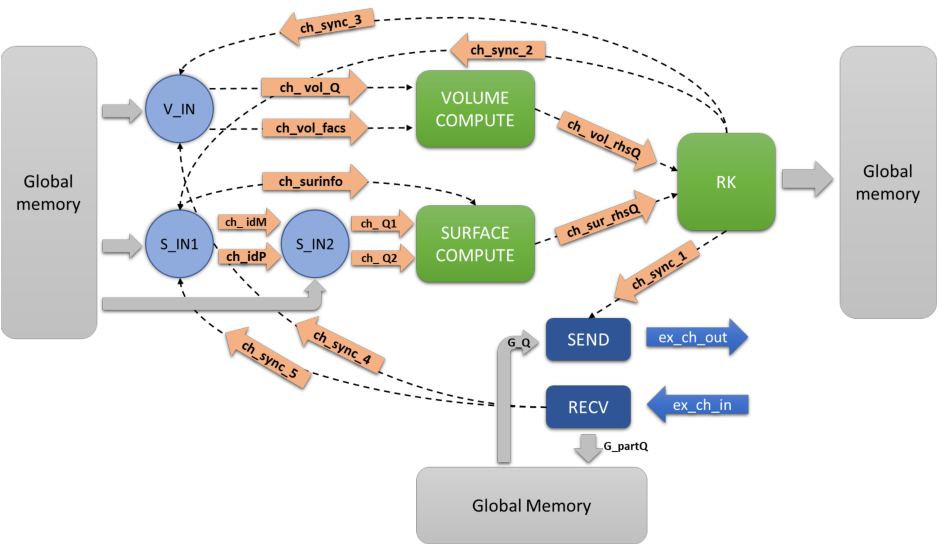
\includegraphics[width=1.0\textwidth]{images/channelssync_kernstruc}
    \caption{Kernel structure for FPGA only design utilizing 5 blocking channels for synchronization}
    \label{fig:channelsync_kernstruc}
\end{figure}

In the design, \texttt{ch\_sync\_1} between RK kernel and the send kernel is to synchronize
the start of communication at the beginning of each iteration. \texttt{ch\_sync\_2} and
\texttt{ch\_sync\_3} is used to synchronize the completion of writing last element into
the memory to start of reading the elements in the next iteration by the input kernels.
\texttt{ch\_sync\_4} and \texttt{ch\_sync\_5} is used to synchronize the completion
of communication from the \texttt{recv} kernels. Though the required sequence of operation
was achieved with the channels and speed up was noticed, the design didn't produce correct
results which was identified due to large deviation in the analytical and the computed
nodal error values. After further analysis of the design it was noticed that the
\acl{LSU} in input kernels used cached access for \texttt{g\_Q\_ping} and \texttt{g\_Q\_pong}
buffer reads which could be a problem with the updated design. As the buffer is updated by the
RK kernel and the kernels are suppose to switch the buffers in each iteration, cached reads
could lead to processing of stale values resulting in wrong field computation. To eliminate
the cache for the memories, the buffer parameter were marked as \texttt{volatile} which
as per the documentation allows to remove cached access as well as perform buffer management \todo{add reference for this}
between the kernels to ensure correct sequence of reads and writes.

\subsection*{Addition of latency}

Another probable issue with the design was with the difference in latency of memory operation
and channel communication. As the channels are implemented as FIFOs in the hardware
using registers or BRAMs, the latency of the channels is much lesser then that of a memory
operation. This would cause the input kernels to assess non-updated memory after receive of the
event over the channels. As shown in the image \ref{fig:memchan_latency}, due to higher latency
of the memory to handle the write request which is not visible in the kernel, an overlapped
read is possible while using channels for synchronization.

\begin{figure}[ht]%
    \centering
    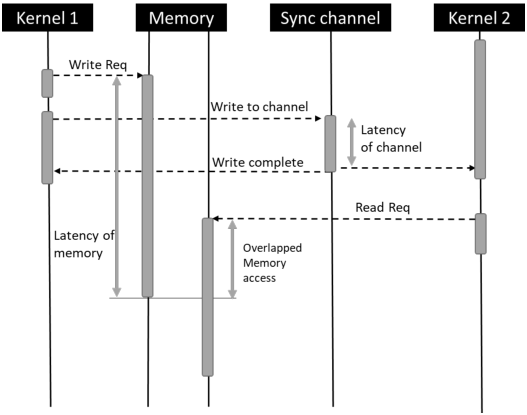
\includegraphics[width=0.6\textwidth]{images/memchan_latency}
    \caption{Sequence of operation between kernels using memory and channels showing
    the latency differences for memory and channel and its effect while using
    for synchronization}
    \label{fig:memchan_latency}
\end{figure}

As there is no concrete information available for the target board to estimate
the latency difference,

\subsection{Synchronization using locks with atomic memory operations}

\section{Final Kernel structure}
\label{sec:final_struc}

\section{Issues identified with optimized design}